\title{
    Temperature Monitoring Network\\
    02220 Distributed Systems 
}
\author{
        Justas Poderys \\
        s120944
        \and
        Hans-Jacob S\o rensen Enemark \\
        s122509	
}             

\date{May 27, 2013}

\documentclass[12pt]{article}
\usepackage[left=2cm,right=2cm,top=3cm,bottom=3cm]{geometry}
\usepackage[square,numbers]{natbib} % citations
%\usepackage[T1]{fontenc}
%\usepackage{lmordern}
\usepackage{graphicx}
\usepackage{caption}
\usepackage{subcaption}
\usepackage{textcomp}
\usepackage{float}
\usepackage{hyperref}
\renewcommand{\paragraph}{\@startsection{paragraph}{4}{0ex}%
   {-3.25ex plus -1ex minus -0.2ex}%
   {1.5ex plus 0.2ex}%
   {\normalfont\normalsize\bfseries}}
\makeatother
\frenchspacing

\stepcounter{secnumdepth}
\stepcounter{tocdepth}

\begin{document}
\maketitle
\setcounter{tocdepth}{2}
\newpage
\tableofcontents
\newpage

%Main part of report
\section{Introduction}
\label{sec:intro}

Sometimes grasping the big picture of a situation means piecing it together from very small parts. This could be as diverse as how a structure is reacting to an earthquake, the currents movements in the oceans, the change of weather in an entire country or something as volatile as the conditions inside a tornado.
Even though the conditions and situations are different it all boils down to collecting specific data from individual locations at certain time intervals and then process it for further study.

In order to deliver each datapoint it is necessary to set up a certain type of infrastructure and software architecture. This comprises a medium through which the data is to be send and a piece of software to handle the sending and recieving of the data - the middleware.

This project is focused on the middleware. With a layered approached this middleware will seperate the data transfer and the coordination into two different parts. This way the transport medium could be replaced to fit the context of the application. In the given situation the data transfer layer will use TCP as a reliable channel.

In the context of monitoring the temperature in a given situation the data is the temperature value and its origin - time and place. The 'place' in this project is the ID of the sensor that captured the temperature value. 

Each sensor node will be able to take one of two roles - normal or admin. In \textit{normal} mode the node sends out the data periodically, and in \textit{admin} mode the data is collected and organised. A 3$^{rd}$ role in the system is the \textit{user} who can request the average temperature from the current admin node and promote a normal node to admin. 

The goal of this project is to get a current status of the temperature in a fictive scenario using distributed concepts. 
The proposed sulution is designed for a Linux context and implemented using the C programming language. 
 

\section{Proposed solution}
\label{sec:proposedsolution}
With the objective of monitoring the temperature of a given area - e. g. a piggery, the scenario is as follows: A number of similar sensor nodes is distributed around the area each connected to the same network. This network is in this project capable of providing a reliable channel through TCP. A \textit{user}-entity chooses one sensor node to be the admin node. 

As depicted in Figure \ref{fig:overview} the execution of the system can be devided into 3 main categories:
\begin{description}
    \item[Reporting] Regular nodes reports their temperature to the admin node periodically.
    \item[User request] Upon request, the admin node evaluates the average temperature from the available data that is not too old and returns the result.
    \item[Promote new master] When an admin node crashes or other wise fall out of service, the user then selects and promotes a regular node, which in turn notifies the remaining regular nodes of the promotion.
\end{description}
\begin{figure}[ht!]
\centering
    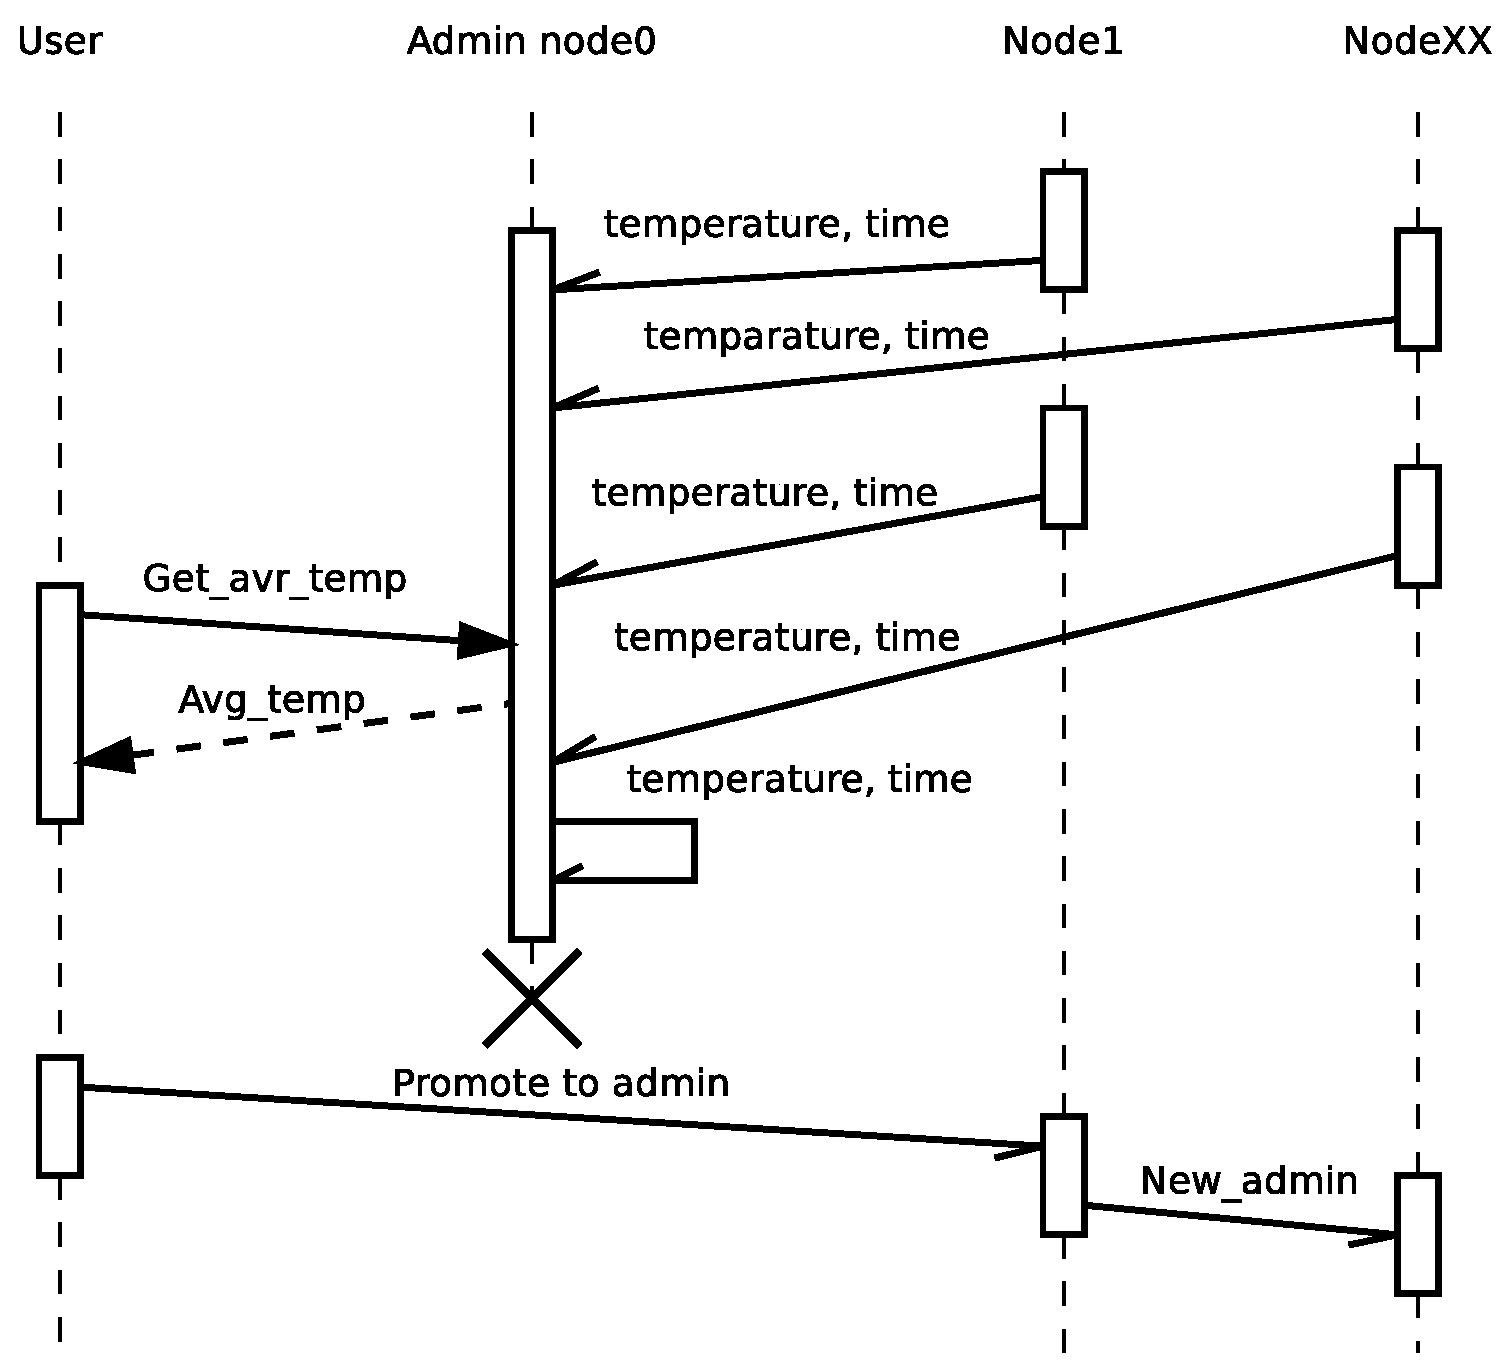
\includegraphics[scale=0.4]{eps/communications2}
\caption{The most prominent messages in the system}
\label{fig:overview}
\end{figure}
\subsection{Assumptions}
\label{subsec:assumptions}
The following assumptions are made about the context of the system:
\begin{itemize}
    \item All nodes are syncronized within a certain margin. This is done to be able to timestamp each temperature value and provide the user with an up to date picture of the temperature situation. 
    \item Reliable channels. Using the TCP protocol each data point is assumed delivered after it has been sent. % [Come up with a justification]
    \item Secure channels. No data is corrupted or generated by outsiders with malicious intend.
    \item Data integrity. The data received is assumed to be the data that is sent. No data is generated out of nowhere.
    \item IP addresses of all nodes are known to the user in before deployment of each node.
    \item Channels are asynchronous and message can take arbitrary time to arrive.
    %\item mode assumptions...?
\end{itemize}

\section{Design}
\label{sec:design}

In the overall design a modular approach has been chosen. This is done to devide the code into logic pieces, each with a clear cut role - much similar to the object oriented style from C++ or Java. Following this pattern makes the code easier to grasp - and to re-use for future use.

%The connections on the network will be set up using sockets in C. The sockets will use TCP as a reliable transfer protocol. This way any message is assumed delievered once sent. 

To keep the system going the messages are passed between the sensor nodes and the user. These messages are showvn in Figure~\ref{fig:messages}.
\begin{figure}[ht!]
\centering
    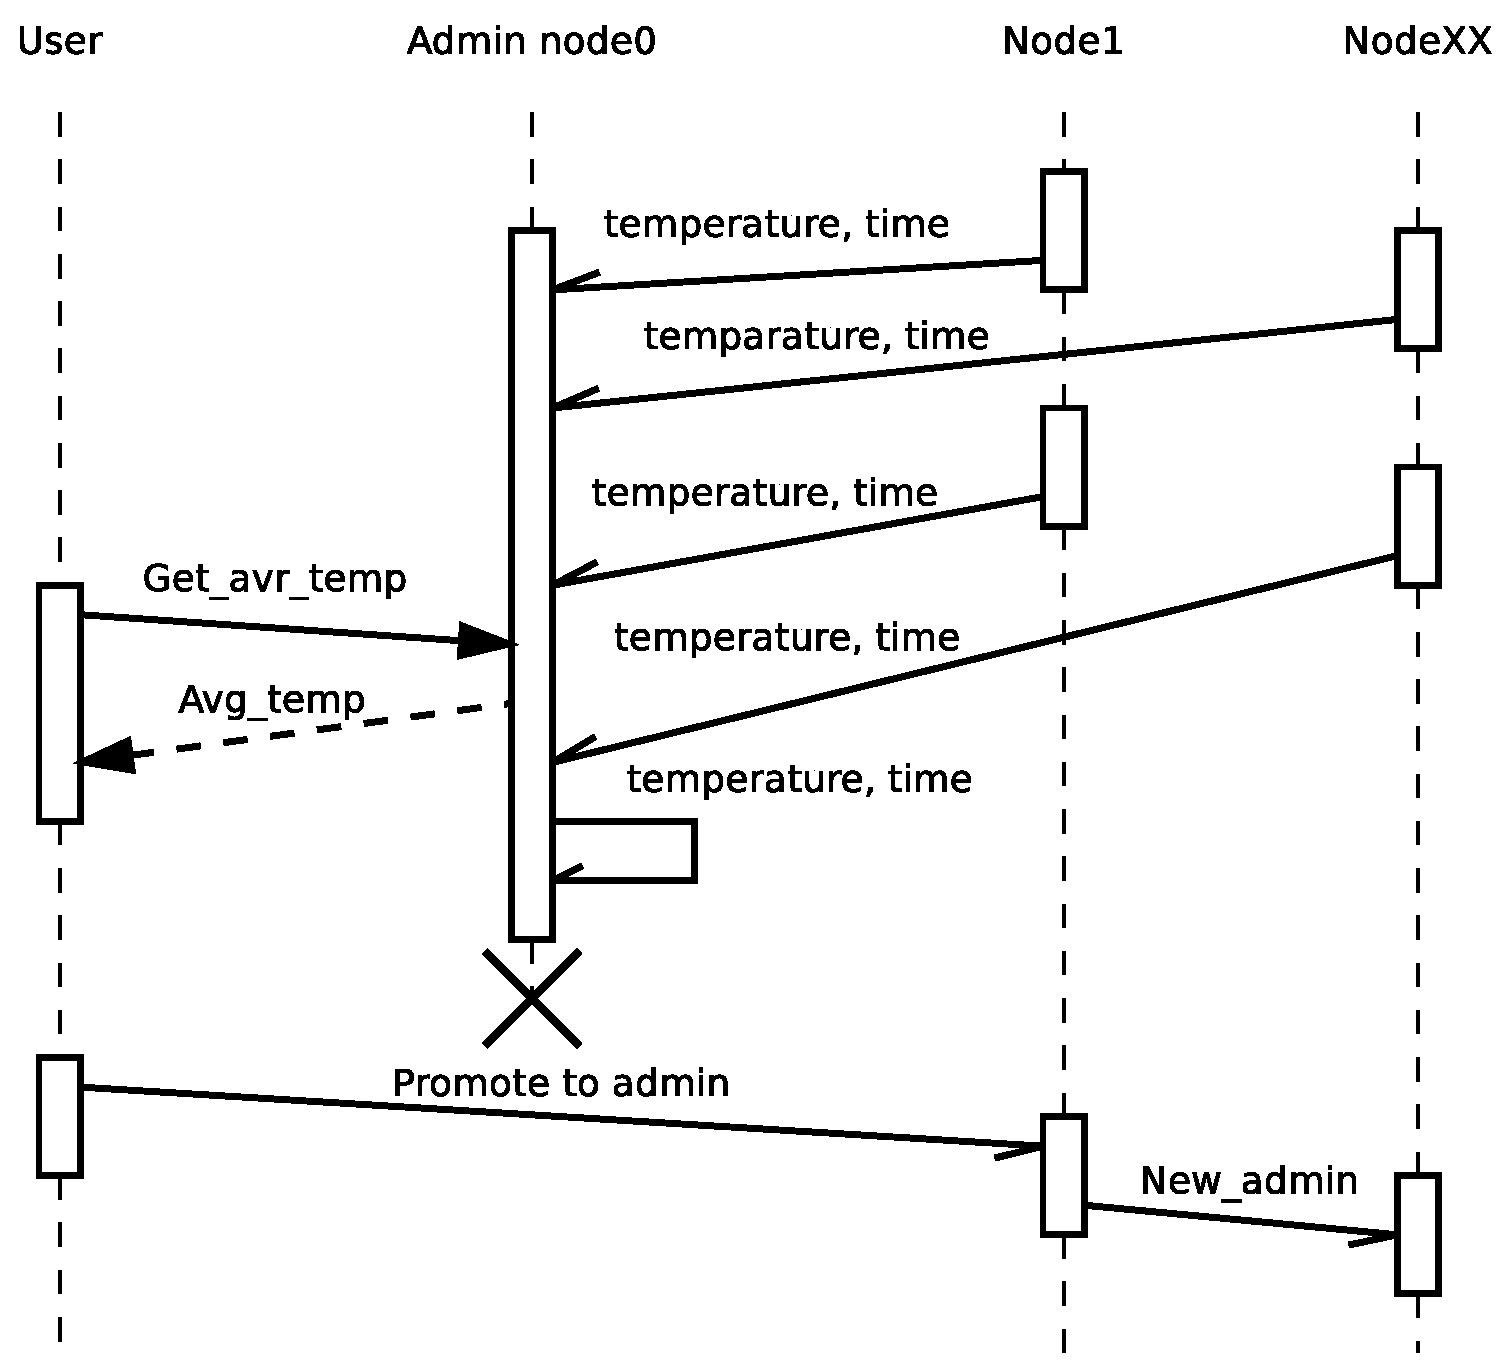
\includegraphics[scale=0.4]{eps/communications2}
\caption{Messages in the system}
\label{fig:messages}
\end{figure}

These messages are sent using \textit{exactly once} semantics, through TCP. This way the application level software only has to hand over the message to the transport layer and it will be sent reliably.

As it is shown in Figure~\ref{fig:messages} every node has to fill the role as a sensor. That means that the admin node has to have two roles. To achieve this the sensor software is devided into three parts - one for each of the jobs mentioned in section \ref{sec:proposedsolution}. With a clear seperation it is possible for the admin node to send temperature data to itself and thus keep working with two roles.

Special care must be given to the fact that there might be several master nodes operating at the same time. This can happen when first master node goes down and next node is promoted to be a master node. In the case that first master nodes comes up thinking that it is still a master node, there will be a situation with two master nodes working at the same time. To provent this each promotion to master node from simple node carries a pormotion key. Promotio key is increased by user node each time new promotion is done. When master nodeannounces itself to be a master node by broadcasting this information, it includes master key in a announcment. If temperature node receives announcment from a node with a master key lower than current configured, this announcment will be ignored.

%%%%%%%%%%%%%%
%%%% The following might be implementation description ...?
%%%%%%%%%%%%%%

\section{Implementation}
\label{sec:implementation}
In the following relevant implementation details will be discussed for each of the main parts of the system. 

The software is to be written using the C programming language. This choice is made based on the familiarity with the language and freedom it provides. Using this language makes the transition into a real world scenario with an embedded platform as the heart of the sensor rather trivial. 
\subsection{Sensor node with dual roles}
\label{subsec:sensornodedesign}
The dual role functionality requires threads, with each thread to handle a particular task these threads are described in Figure \ref{fig:sensorthreads}. One main thread spawns the other threads and is left out. With this structure a node can take two roles - both collecting temperature data and send it to the admin, and receiving data as an admin and process it. Thus sending data to itself as needed.

\begin{figure}[ht!]
\centering
    \begin{subfigure}[b]{0.3\textwidth}
        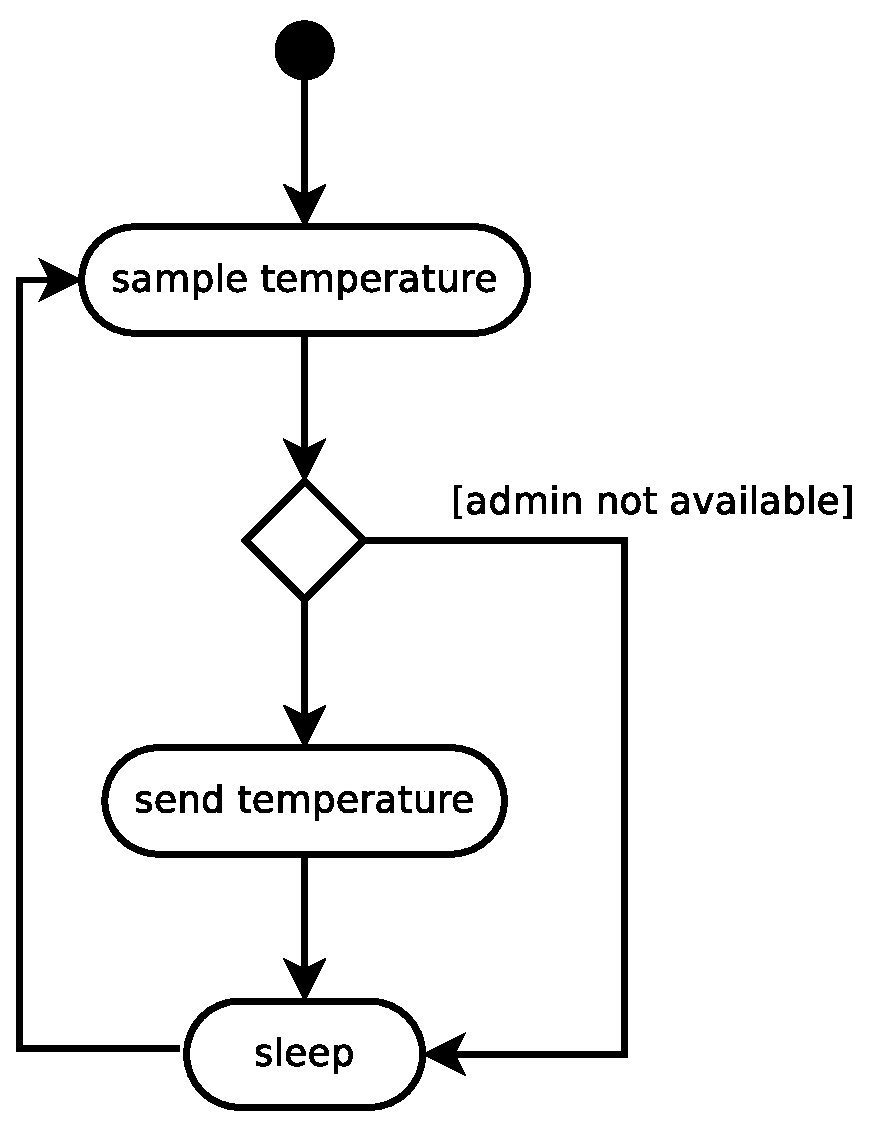
\includegraphics[scale=0.35]{eps/temp_th}
        \caption{Temperature thread}
        \label{fig:tempthread}
    \end{subfigure}
    \begin{subfigure}[b]{0.3\textwidth}
        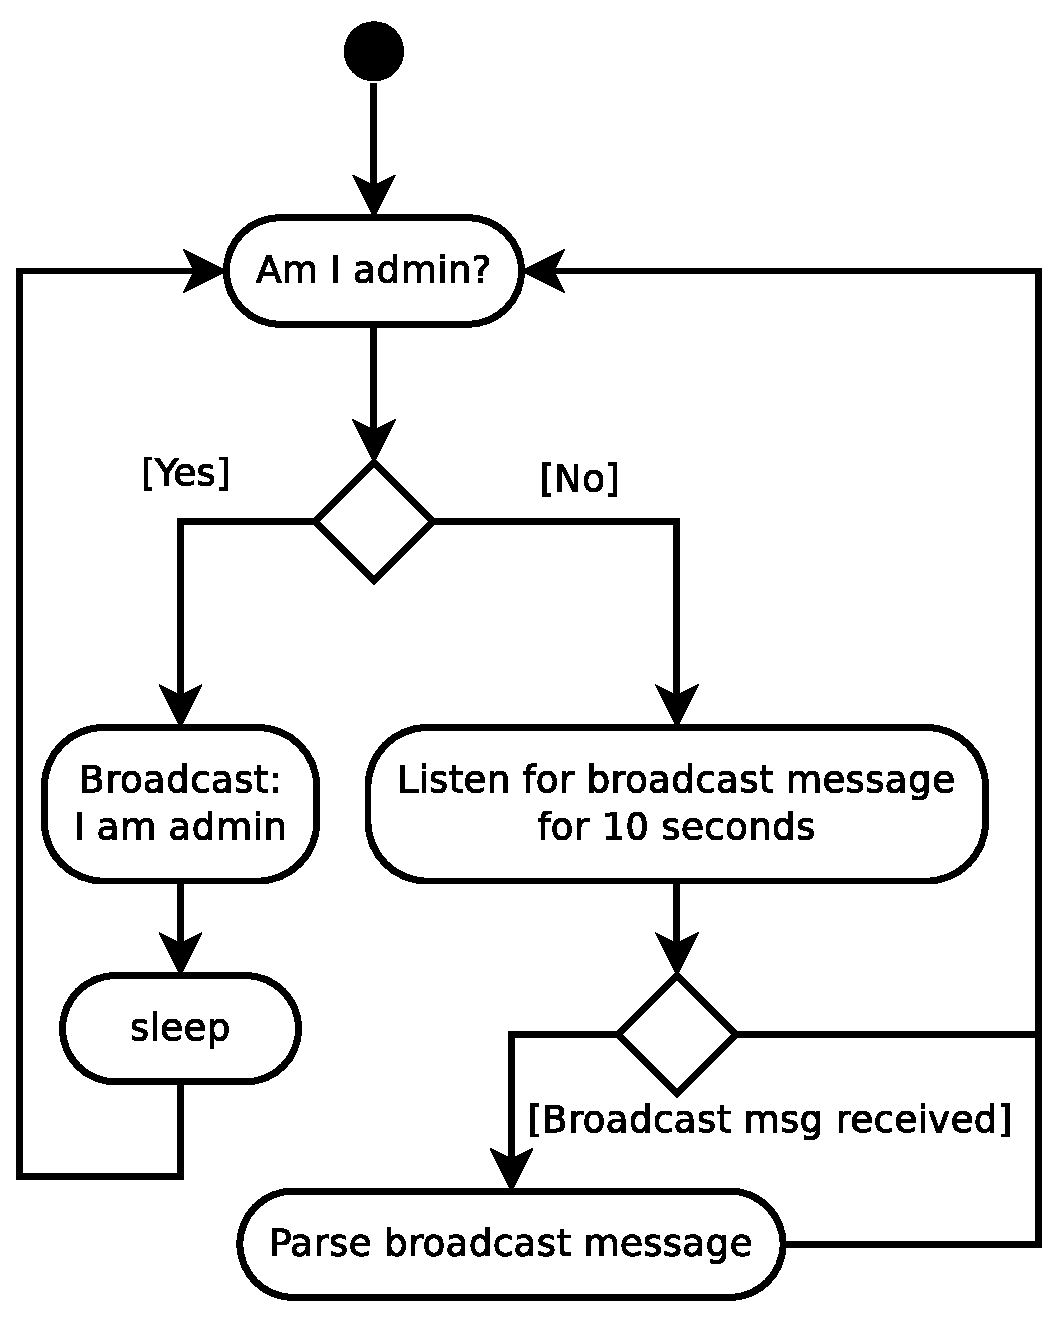
\includegraphics[scale=0.35]{eps/admin_th}
        \caption{Administrator thread}
        \label{fig:adminthread}
    \end{subfigure}
    \qquad
    \begin{subfigure}[b]{0.3\textwidth}
        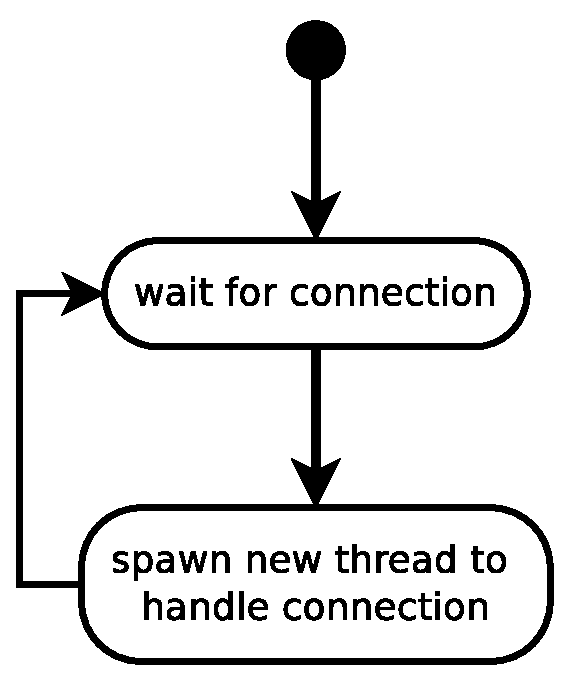
\includegraphics[scale=0.35]{eps/data_th}
        \caption{Data handler thread}
        \label{fig:datathread}
    \end{subfigure}
    \caption{Flow charts on each thread in the sensor}
    \label{fig:sensorthreads}
\end{figure}

\subsection{User entity}
\label{subsec:userdesign}
The user piece of software is a straight forward command line tool. Listing the available options with numbers provides the user with a way to interact with it. Interaction is done by entering a number corresponding to the function and pressing the return key. Main functions are:
\begin{enumerate}
    \item \textbf{Quit:} Ends the program.
    \item \textbf{Connect to node:} Asks for an IP address and opens a connection to that IP.
    \item \textbf{Promote to Admin node:} Initiates the promotion process on the selected node. The admin node is provided a key, that is unique to the admin.
    \item \textbf{Get average T from node:} Requests the average temperature from the available data on the admin node.
\end{enumerate}
The main structure of this program is a simple while()-loop that prints out the menu-options and waits for input on \textit{stdin}. When an input is provided, a switch case evaluates the input and acts accordingly.

\subsection{Message Passing}
\label{subsec:msgpassing}
To transfer messages between the node IP protocol is used. On top of IP protocol, TCP and UDP protocols are used for connection management. TCP protocol is used to provide reliable message passing between user and nodes in the system and between nodes themselves. UDP protocol is used to provide broadcast communications. Due to the fact that UDP protocol does not guarantee delivery of messages, broadcast messages are repeated at set time intervals. UDP broadcast solutions was chosen due to the simplicity of implementation.

\subsection{IP Version agnosticism}
\label{subsec:ipveragn}
Implementation of the sensor system is mostly IP version agnostic. It was implemented this way due to the fact that networks are transitioning from the usage of IP version 4 to IP version 6 protocol. Converting the system to be fully compliant with IP version 6 would require minimal changes in source code. The only change that has to be done is to change the IP address that is used for broadcasting. At the moment broadcasts are sent to the local broadcast address. This broadcasting method is not supported in IP version 6. In IPv6 native systems, broadcast messages should be sent to FF02:0:0:0:0:0:0:1 address which is reserved for multicast ``All nodes address'' communication. Decision to leave IP version 4 method of communication was done mainly due to the fact that IPv4 systems were used for testing.

\subsection{Messages format}
\label{subsec:msgformat}
To provide a scalable solution for message passing, Type-Length-Value (TLV) messages format was used. In TLV messages, each message is encoded in a tuple \{Type, Length, Value\}. Type and Length are integers, first one indicating what kind of message it is and second how long is the Value. TLV encoded messages are easy to serialize and deserialize for sending and later can be easily parsed as a linked list, because all types are known beforehand and length of each message is 2 times length of integer plus value of Length integer. If new message type has to be added, it is enough to add new Type value and update message parsing code with new message type. Serialization, deserialization and parsing code is same regardless of place where it is used - user node, sensor node or master node.  

\subsection{Time offset calculation}
\label{subsec:timesync}
It is assumed in the system model used, that the communication channels are asynchronous. In temperature monitoring system this means that temperature value read in one node can take arbitrary time to reach master node. To solve this issue, time offset calculation is done. When node learns about new master node, it calculates the time offset from node local clock to the master local clock. This time offset then is used to adjust the local timestamp when reporting time when temperature reading was done to the master node. Further more, because all temperature values are timestamped with admin local time, it is easy for admin node to discard old messages. Time offset calculation is done using Network Time Protocol on-wire protocol \cite{ntpv4_standard}. Ilustration of this protocol is provided in Figure~\ref{fig:timeoffset}
\begin{figure}[ht!]
\centering
    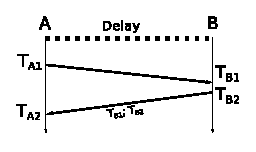
\includegraphics[scale=1]{eps/NTP_onwire_diagram}
\caption{Offset calculation protocol}
\label{fig:timeoffset}
\end{figure}

Protocol operation starts when peer A sends packet at time $T_{A1}$ to peer B. Upon reception of this packet, node creates timestamp when packet was received $T_{B1}$. Then it constructs the reply packet. Receive timestamp is time when packet was received at a server $T_{B1}$. Finally transmit timestamp $T_{B2}$ is added just before sending packet back to peer A. Upon reception of this reply message, peer A creates a timestamp $T_{A2}$ to indicate when packet was received. At this point peer A will calculate offset 

$\theta=\frac{(T_{B1}-T_{A1})+(T_{B2}-T_{A2})}{2}$

This offset is later used to adjust local timestamp when sending messages to master node.

\subsection{Threading}
\label{subsec:threading}
Temperature sensors in this project are implemented using POSIX-threading (Pthreads). Pthreads are used to provide logical separation of tasks in each node. There are separate threads for data messages handling, temperature handling and broadcast messages handling. Using pthreads allowed to achieve error separation (error in one thread logic, will not affect other thread) and also easier workload distribution between programmers. Second place where pthreads are used is handling of multiple connections. Many application written in C use fork() system call to handle connection, but this was not an option for this implementation, because of the need of global variables visible from all threads.
\label{subsec:msgpass}

\section{Test of the system}
\label{sec:testing}
In the following first the key test setup and then the main test objectives is described.

The sensor network is tested in a Linux environment on two laptops running Ubuntu. These two laptops are interconnected with an ethernet cable. For further details on the setup see \ref{subsec:testsetup}.

The testing is done to document that the functionality is as expected and acts as outlined in the project description. To test this, the following steps is executed:
\begin{enumerate}
    \item A number of instances of the sensor program is started
    \item The user program is started seperately.
    \item Promote one sensor to admin.
\end{enumerate}
This scenario will test that everything works initially and that every part of the software runs. 
After this startup procedure a random non-admin node is stopped and started again to show that it will find the admin node again. Then the admin node is stopped and a new one is promoted, to show that the sensor nodes can switch admin node without userinteraction.

This will show a working system that fulfills the requirements outlined in the project description.


\section{Conclusion}
\label{sec:conclusion}

During a time of this project, a temperature monitoring and data gathering solution was implemented. Solution is designed to work in a distributes monitoring enviroment and to cope with simple failures - like delayed messages or several admin nodes working at the same time. Solution was implemented using a C programming language and a PThreads library for workloads separation. Command line user interface program was also implemented to promote nodes to master state and later to get average temperature readings. Solution was tested on two computers connected by Ethernet connection and each computer running 3 sensor nodes. No deviation from specification was noticed during a testing runs of a system.

\subsection{Responsibilities}
\label{subsec:responsebilities}

Program was written by both students. Data storrage, access, filtering and updating functions were written mostly by Hans-Jacob and network sockets processing was mostly written by Justas. Final report was a joint work of both Hans-Jacob and Justas.

%the rest of it
%\bibitem{ntpv4_standard}
	D.Mills et.al.
	Network Time Protocol Version 4: Protocol and Algorithms Specification, 
	Request for Comments: 5905
\label{totalpage}
%% For bibliography %%
%
\bibliographystyle{unsrt} % these / plain / alpha / unsrt / abbrv (http://amath.colorado.edu/documentation/LaTeX/reference/faq/bibstyles.html)
\bibliography{sources}
\label{biblo}
\newpage
\appendix
\section{Test setup and execution}
\label{sec:appendixtest}
\subsection{Test setup}
\label{subsec:testsetup}
To prepare a computer for testing the sensor network it is necessary to setup extra network interfaces. In Ubuntu this is done with the following command:
\begin{quotation}
    $\sim$\# ipconfig eth0:x $<$new\_ip$>$ netmask $<$netmask$>$
\end{quotation}
In this situation the ethernet port \texttt{eth0} is used for the testing and only because it is not used for anything else. The \texttt{x} is the desired number for the new pseudo interface. \texttt{new\_ip} is the desired new IP address and the \texttt{netmask} is the netmask used. In the test one interface was set up using the following command: 
\begin{quotation}
    $\sim$\# ipconfig eth0:1 10.10.10.1 netmask 255.255.255.0
\end{quotation}

This command is executed as many times as desired to form the basis for the test.

\subsection{Test execution}
\label{subsec:testexecution}
After the preparations is done it is now possible to run a number of instances of the \texttt{sensor} program. Each instance is tied to one interface, hence the number of interfaces is the maximum number of possible instances. The \texttt{sensor} is executed with the following command:
\begin{quotation}
    $\sim$\# ./sensor v4 $<$ip$>$
\end{quotation}
Where \texttt{ip} is any of the available IP adresses set up earlier and \texttt{v4} indicates that an IPv4 address will be provided.

The following will describe a number of test cases to show the functionality of the system.
\subsubsection{Start up}
\label{subsubsec:startuptest}
Whith the sensor instances running one \texttt{user} is needed to promote one sensor node to admin. This is done with the following:
\begin{enumerate}
    \item Start the user
        \begin{quotation}
            $\sim$\# ./user
        \end{quotation}
    \item Enter \texttt{2} for Connect to node.
    \item Enter IP address of a sensor node.
    \item Enter \texttt{3} for Promote node.
\end{enumerate}
After this test a number of sensor nodes is running of which one has been promoted to admin node and the user program is running.
\subsubsection{Adding a sensor node to the network}
\label{subsubsec:addingnodetest}
This test assumes completion of section \ref{subsubsec:startuptest} and a running sensor network with the admin node functioning. 

The only step in this test is to start up a new instance of the sensor program and see that it finds the admin node and starts transmitting temperature data.

\subsubsection{Getting a new admin node}
\label{subsubsec:newadmintest}
This test assumes completion of section \ref{subsubsec:startuptest}.
\begin{enumerate}
    \item Stop the admin node instance
    \item With the user promote another sensor to admin node as in section \ref{subsubsec:startuptest}.
\end{enumerate}
All working sensors will now receive the broadcast message from the new admin node and start transmitting data to the new admin.

\subsubsection{Fetching the average temperature of all nodes}
\label{subsubsec:fetchtemptest}
This test assumes completion of section \ref{subsubsec:startuptest}. All interaction in this test is done with the user program.
\begin{enumerate}
    \item Enter \texttt{2} for Connect to (admin) node.
    \item Enter IP address on the admin node.
    \item Enter \texttt{4} for Get average T from node.
\end{enumerate}
The user should now see a temperature value in the terminal.
\subsection{Test output}
\label{subsec:testoutput}

---- put test output here ----

%\bibitem{ntpv4_standard}
	D.Mills et.al.
	Network Time Protocol Version 4: Protocol and Algorithms Specification, 
	Request for Comments: 5905
\end{document}
